\chapter{Data Preparation}\label{sec:data}

This study is based on simulated data produced with GEANT4~\cite{GEANT4}, using the geometric layout of the proposed Linear Collider Detector (LCD) for the CLIC accelerator~\cite{Lebrun:2012hj}. We limit the study to the central region (barrel) of the LCD detector, where the electromagnetic calorimeter (ECAL) consists of a cylinder with inner radius of 1.5 m, structured as a set of 25 silicon sensor planes, segmented in $5.1~\times~5.1$ mm$^2$ square cells, alternated with tungsten absorber planes. In the barrel region, the hadronic calorimeter (HCAL) sits behind the ECAL, at an inner radius of 1.7 m. The HCAL 
consists of 60 layers of polystyrene scintillators, segmented in cells with  $3~\times~3$ cm$^2$ area and alternated with layers of steel absorbers. 

The event simulation considers the full detector layout, including the material in front of the calorimeter and the effect of the solenoidal magnetic field. The inner tracker is included in simulation, which allows particles to interact before hitting the calorimeter, but in our studies we focus only on calorimeter data. From the full data for each event we take slices centered around the barycenter of each ECAL energy deposit (including the HCAL), and we represent the ECAL and HCAL slices as 3D arrays of energy deposits in the cells.

\section{Data Contents}

For these studies, we use four kinds of particles (electrons $e$, photons $\gamma$, charged pions $\pi$, and neutral pions $\pi^0$) with energies uniformly distributed between 2 and 500 GeV, and with incident angles uniformly distributed within a polar angle $\theta$ of 1.047 to 2.094 radians with respect to the beam direction (equivalently, a pseudorapidity $\eta$ between -0.549 and 0.549).

To calculate the barycenter of a shower, we take the 2D projection of the shower energy deposit on the ECAL inner surface. This projection is taken along the z direction, which runs perpendicular to the calorimeter surface. Then, using the polar coordinates of the shower barycenter, we estimate the particle's polar and azimuthal angles $\theta$ and $\phi$. The estimated pseudorapidity $\eta$ is then computed as $\eta=-\log[\tan\left(\frac{\theta}{2}\right)]$. Each single-shower event is prepared by taking a slice of the ECAL in a window around the shower barycenter, as well as the corresponding HCAL slice above. For the two tasks (generation and reconstruction), we have produced the following datasets:

\begin{itemize}
    \item {\bf GEN dataset}: A $51 \times 51 \times 25$ cell window in the
    ECAL, for electrons in the energy range $100-200$ GeV. Used in the shower generation task.
    \item {\bf REC dataset}: A $25 \times
    25 \times 25$ cell slice of the ECAL
    and a corresponding $11 \times 11 \times 60$ cell slice of the
    HCAL, for $e,~\gamma,~\pi,$~or~$\pi^0$ in the energy range $2-500$ GeV and with $\eta$ from $-0.524-0.524$. Used in the particle reconstruction task.
\end{itemize}

We have used a larger window for the generation task, in order to capture as much of the shower information as practically possible. For the reconstruction dataset, we reduced the size a bit to reduce memory usage and training times. This is part of why we eventually ended up with a separate GAN framework. We will show in Section~\ref{calo_rec_window_size} that a reduced window size is appropriate for reconstruction tasks.

\section{Data Visualization}

Examples of a photon shower and a neutral-pion shower can be seen in Figure~\ref{fig:sample}. The incoming particles enter from the bottom ($z=0$), at the center of the $(x,y)$ transverse plane ($x=y=25)$. Both events are around 35 GeV in energy. We can see the presence of two subtracks in the neutral pion event, due to decay into two photons.

\begin{figure*}[htbp]
    \centering
    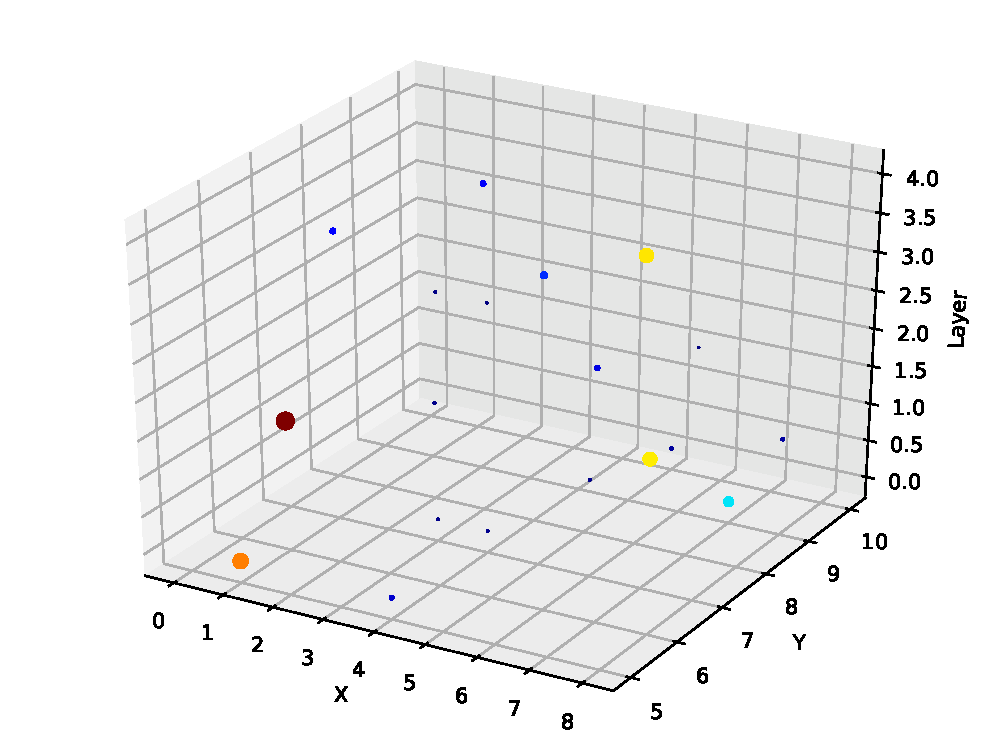
\includegraphics[width=0.45\textwidth]{Images/Calo/Gamma_HCAL.eps}
    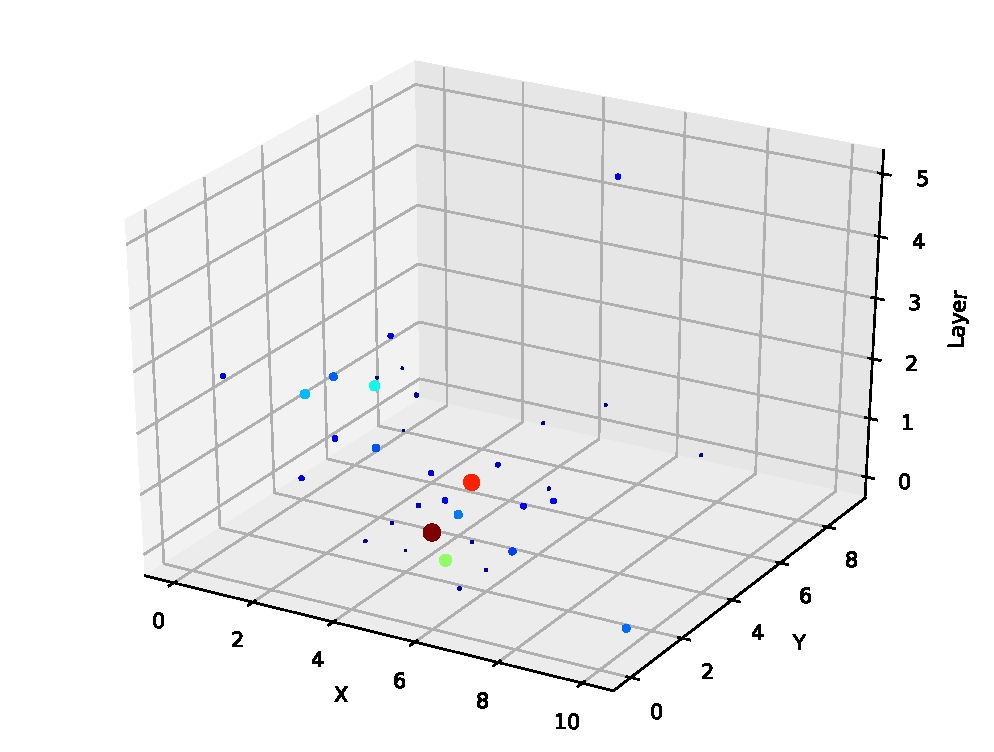
\includegraphics[width=0.45\textwidth]{Images/Calo/Pi0_HCAL.eps} \\
    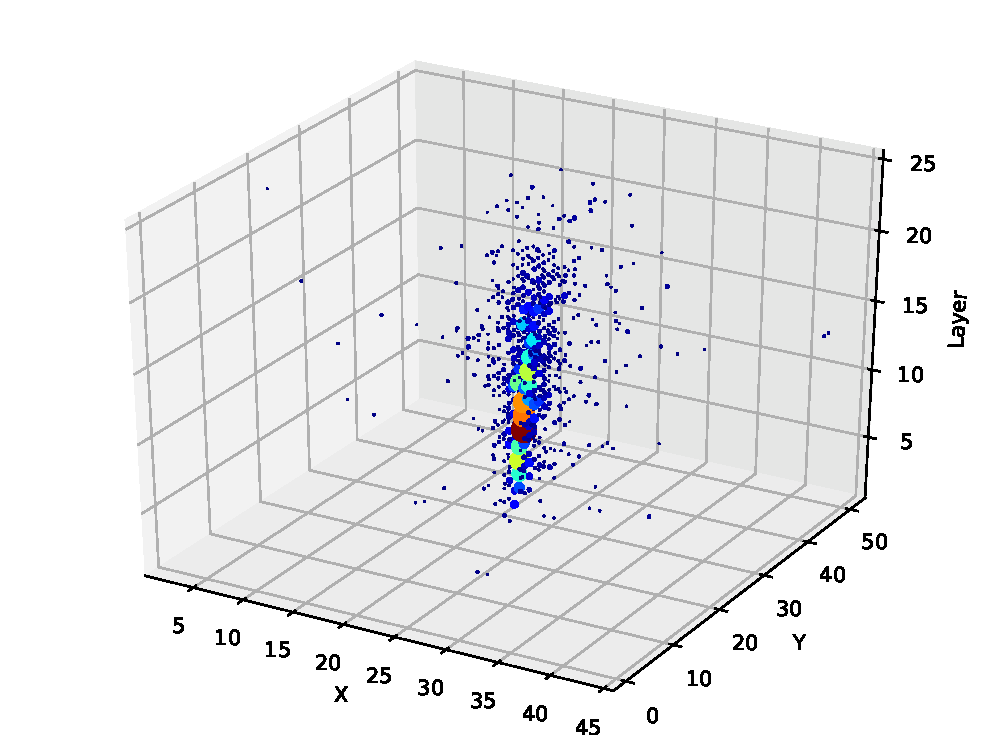
\includegraphics[width=0.45\textwidth]{Images/Calo/Gamma_ECAL.eps}
    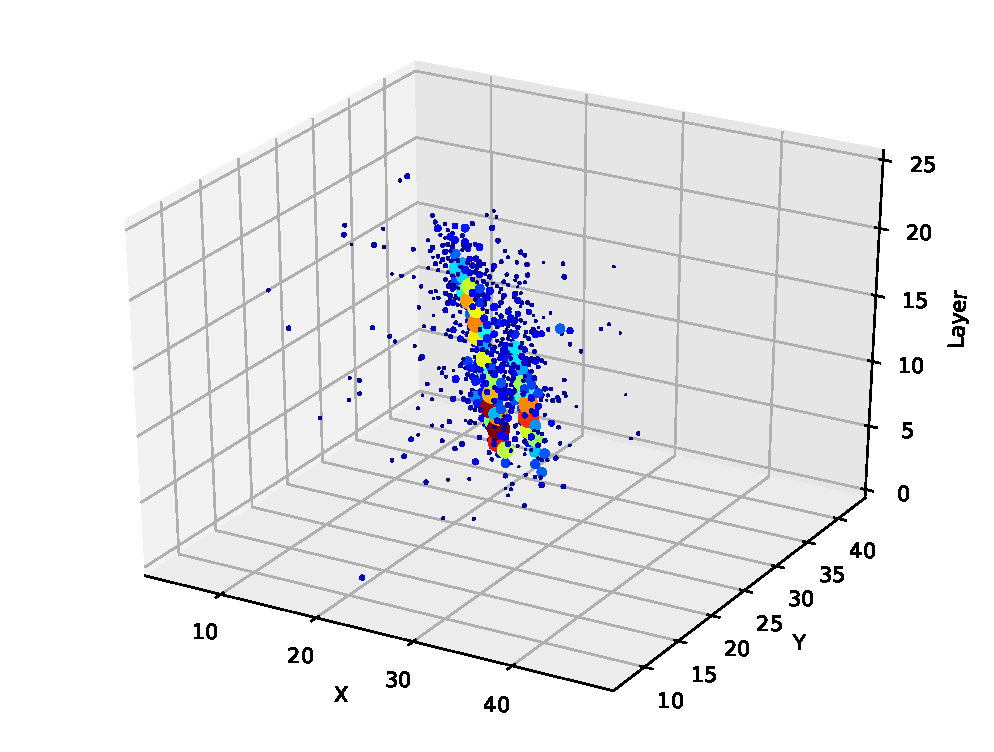
\includegraphics[width=0.45\textwidth]{Images/Calo/Pi0_ECAL.eps}
    \caption{3D image of a photon (left) and neutral pion (right) shower in ECAL (bottom) and HCAL (top).}
    \label{fig:sample}
\end{figure*}

\section{Data Filtering}

We apply a task-dependent filtering of the REC dataset, in order to select the subset of examples for which the task at hand is not trivial. For instance, in general distinguishing a charged pion from an electron is an easy task, and can be accomplished with high accuracy by looking at the HCAL/ECAL energy ratio. On the other hand, a pion with a small HCAL/ECAL ratio leaves most of its energy in the ECAL due to charge conversion processes, and as such would be difficult to distinguish from an electron of equal momentum. Thus, to target the region where a classification algorithm would have most impact, we ignore charged-pion showers with a large HCAL/ECAL energy ratio.

To be more specific, we see in Figure~\ref{fig:HE_ratio} that the ratio of total ECAL energy to total HCAL energy is very different for electrons and charged pions, with the heavier charged pions tending to leave little energy in the ECAL. In order to make the particle-identification task more challenging, we only consider showers with an HCAL/ECAL $< 0.1$ cut. The effects are shown in Figure~\ref{fig:HE_ratio_energy}, where we see the fraction of events from 2-500 GeV that pass this selection. We can see that the selection favors mostly low-energy charged pions, which tend to leave less energy in the HCAL if they manage to make it through the ECAL at all. Discriminating accurately between electrons and charged pions in this range is thus crucial for physics analyses where we are interested in decay products with low energy.

\begin{figure}[htbp]
    \centering
    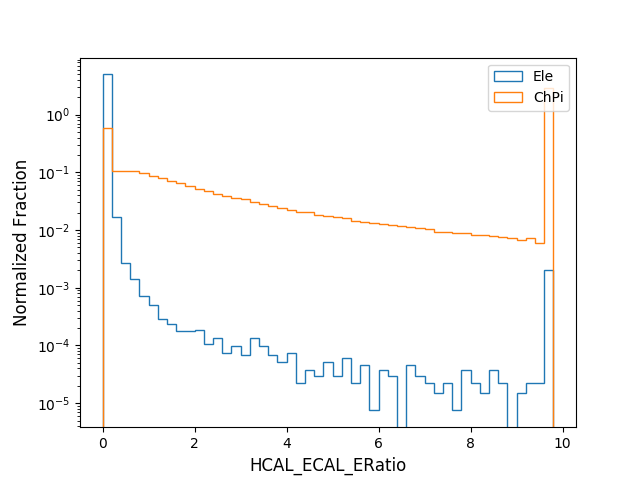
\includegraphics[width=0.7\textwidth]{Images/Calo/ratios.png}
    \caption{HCAL/ECAL energy ratios for electrons and charged pions, plotted on a log scale. The last bin is an overflow bin.}
    \label{fig:HE_ratio}
\end{figure}

\begin{figure}[htbp]
    \centering
    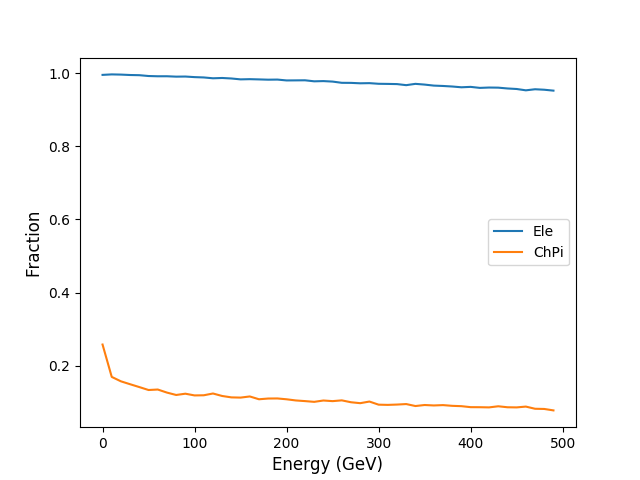
\includegraphics[width=0.45\textwidth]{Images/Calo/ratio_cut_vs_energy.png}
    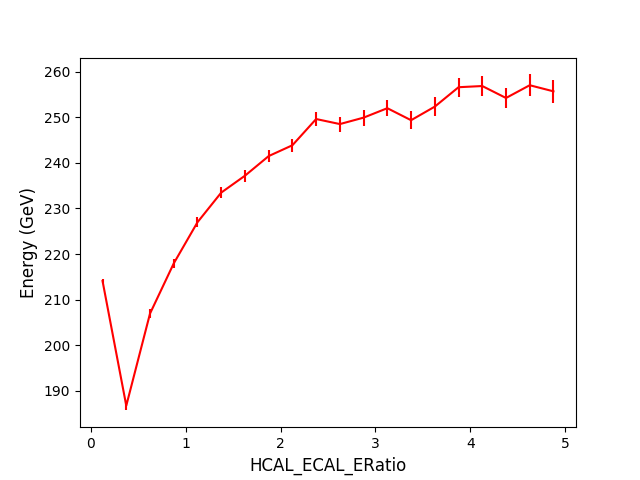
\includegraphics[width=0.45\textwidth]{Images/Calo/mean_energy_vs_ratio.png}
    \caption{Fractions of electrons and charged pions that pass a HCAL/ECAL $< 0.1$ cut at various particle energies (left). Mean charged pion energy as a function of HCAL/ECAL energy ratio (right). We see that if a pion makes it into the HCAL, then we tend to see a positive relation between particle energy and the HCAL/ECAL ratio. About 1 out of 5000 events will leave no hits in the calorimeter window at all, forming the bump in the HCAL/ECAL $= 0$ bin.}
    \label{fig:HE_ratio_energy}
\end{figure}

\begin{figure}[htbp]
    \centering
    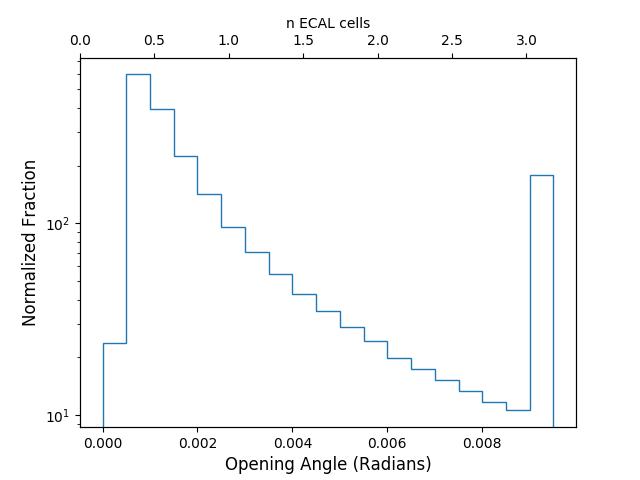
\includegraphics[width=0.7\textwidth]{Images/Calo/zoom_opening_angles.png}
    \caption{Opening angle distribution for neutral pions decaying into two photons, plotted on a log scale with an overflow bin. Plot is zoomed in to show opening angle $< 0.01$. Number of equivalent ECAL cells is shown on the top axis. This plot was generated using pions from the full 2-500 GeV energy range.}
    \label{fig:opening_angle}
\end{figure}

\begin{figure}[htbp]
    \centering
    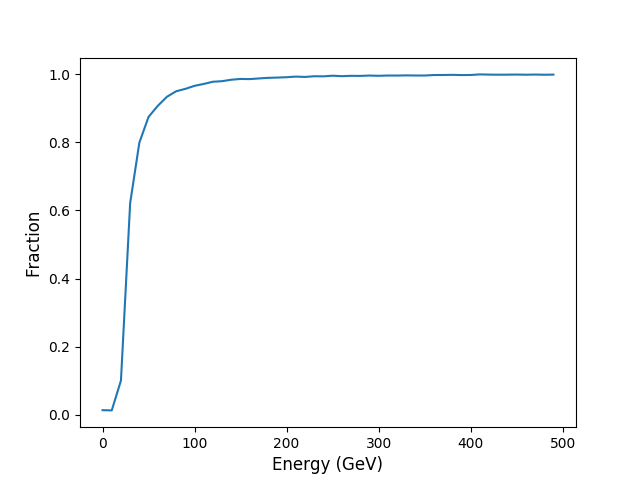
\includegraphics[width=0.45\textwidth]{Images/Calo/opening_angle_cut_vs_energy.png}
    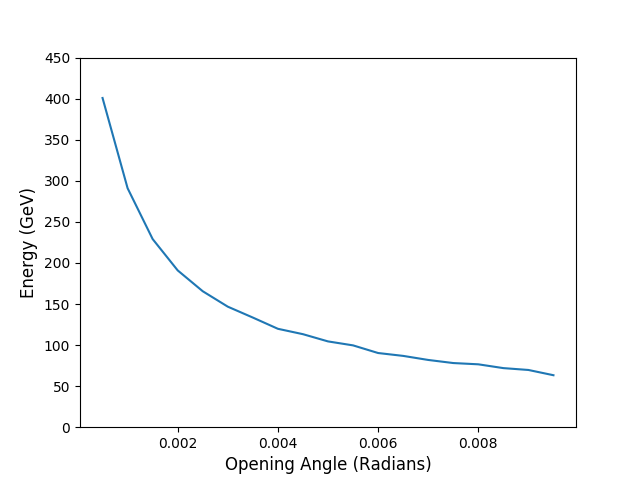
\includegraphics[width=0.45\textwidth]{Images/Calo/mean_energy_vs_opening_angle.png}
    \caption{The fraction of neutral pions passing an opening angle $< 0.01$ radian selection at various particle energies (left). The mean neutral pion energy as a function of opening angle (right).}
    \label{fig:opening_angle_energy}
\end{figure}

Photons and neutral pions are more difficult to distinguish. This is because neutral pions decay preferentially into two photons, with a branching ratio of almost $99\%$. A Lorentz boost due to the momentum of the pion causes the photons to become collimated, to the point where they are only separated by a small angle. If the pion has a low energy, the opening angle between the two photons is larger and the shower is easily identified as originating from a neutral pion. High-energy neutral pions produce more collimated photon pairs, which are more easily mistaken as a single high-energy photon. The opening angle distribution for neutral pions is shown in Figure~\ref{fig:opening_angle}. In order to limit the study to the most challenging case, we filter the neutral-pion dataset by requiring the opening angle between the two photons to be smaller than 0.01 radian.  The effect of  this requirement on the otherwise uniform energy distribution is shown in Figure~\ref{fig:opening_angle_energy}. As expected, the selection mostly removes low-energy neutral pions. 

The ECAL and HCAL 3D arrays are passed directly to our neural networks. We also compute a set of physics-based features, as described in Ref.~\cite{NIPS}. These features are used to train alternative benchmark algorithms representing currently-used ML algorithms in HEP.

\section{Calorimeter Window Size}\label{calo_rec_window_size}

The optimal window size to store for ECAL and HCAL is an important issue, since this impacts not only sample storage size, but also training speed and the maximum batch sizes which we could feed to our GPUs. 

From examinations of our generated samples, we found that an ECAL window of 25x25x25 and an HCAL window of 11x11x60 looked reasonable. To test this hypothesis, we performed training using an unoptimized CNN neural architectures (which will be described later), but with different-sized input samples. The architecture was altered to accommodate larger windows simply by increasing the number of neurons on the input layer. Results trained using an ECAL window of size 25x25x25 and 51x51x25 are shown in Figure~\ref{fig:classification_window}. From the similarity of these curves, we have decided that an expanded ECAL window size does not contain much additional useful information, and is thus not necessary for our problems.

\begin{figure*}[htbp]
    \centering
    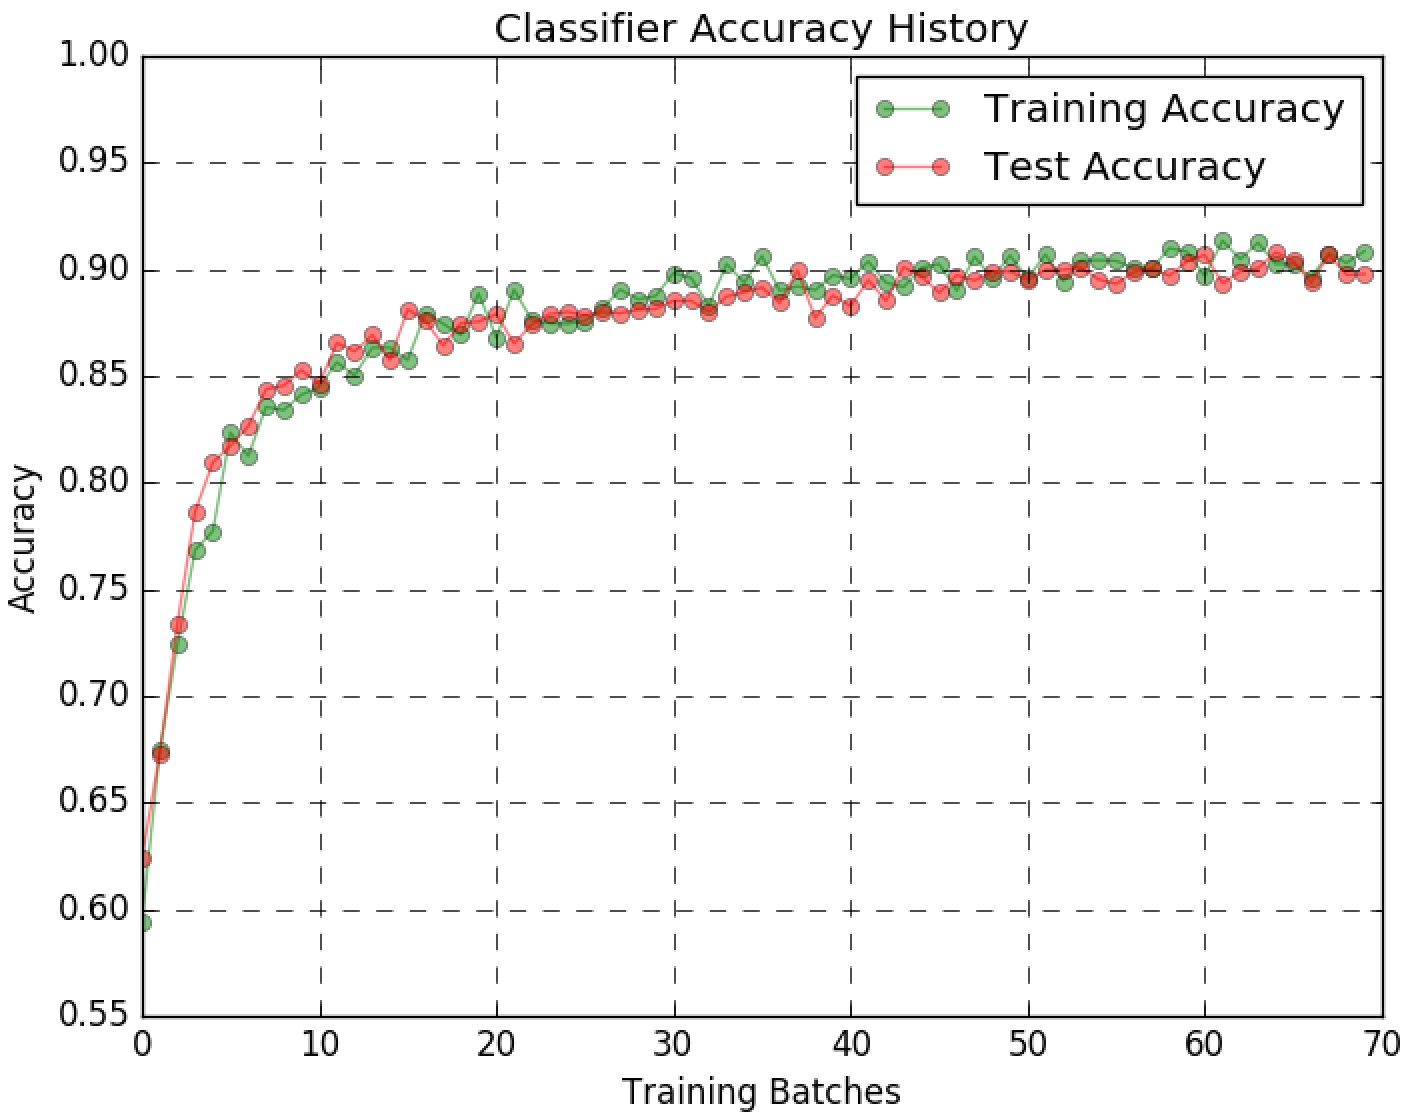
\includegraphics[width=0.45\textwidth]{Images/Calo/accuracy_small_window.png}
    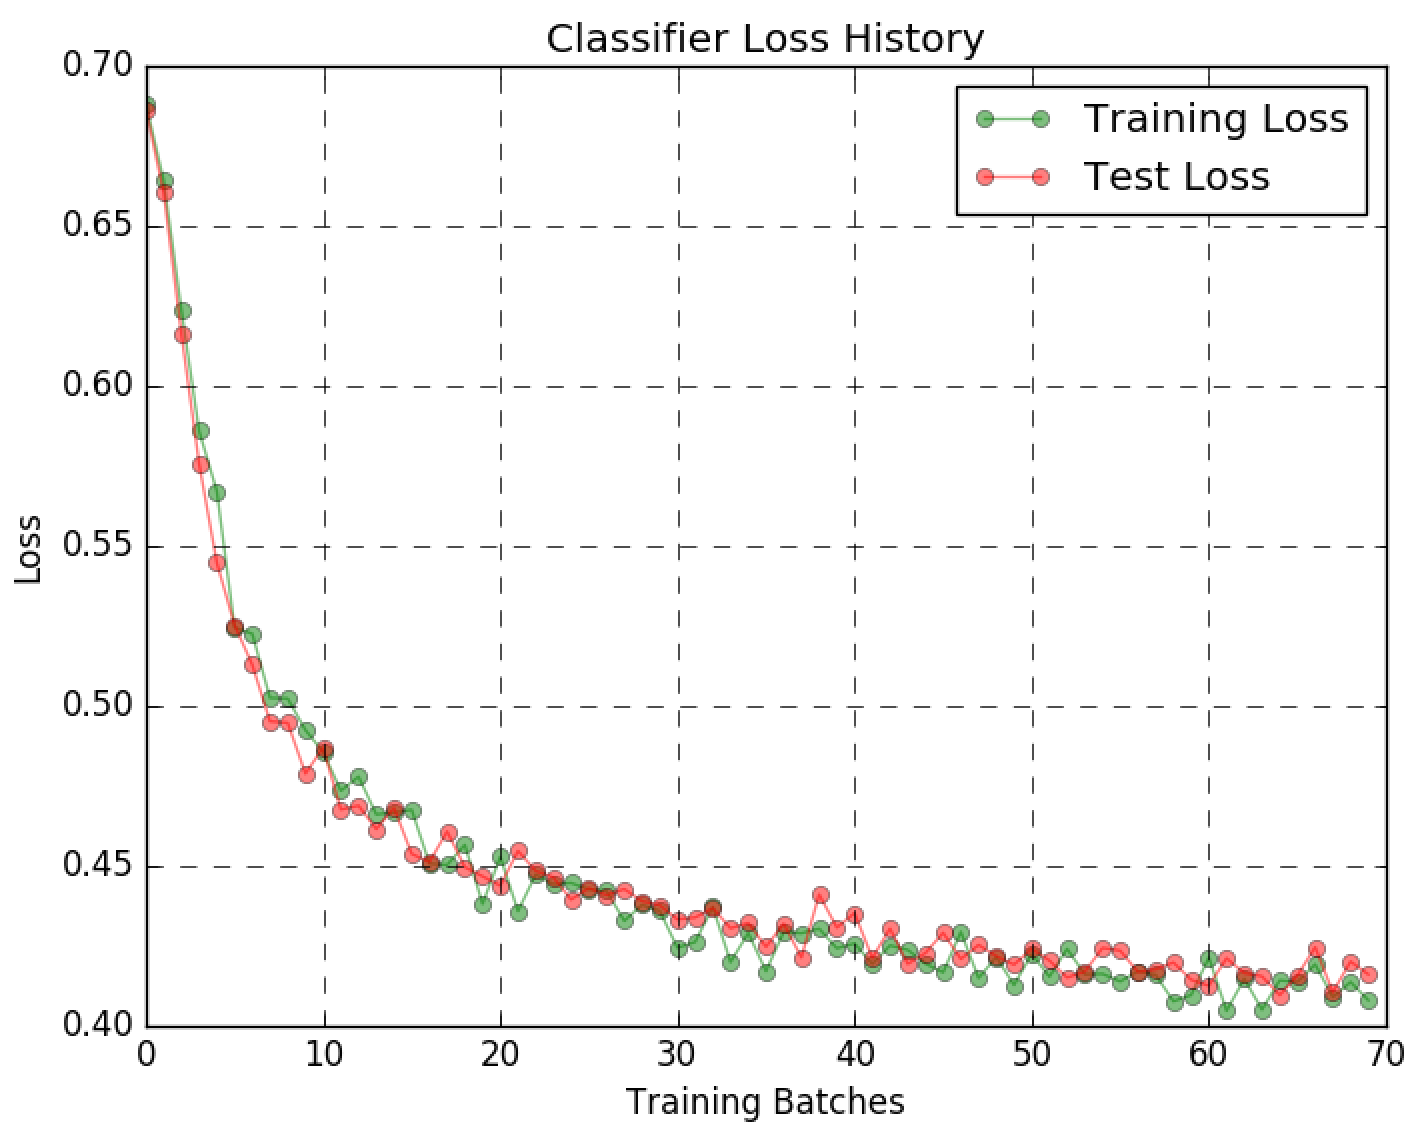
\includegraphics[width=0.45\textwidth]{Images/Calo/loss_small_window.png} \\
    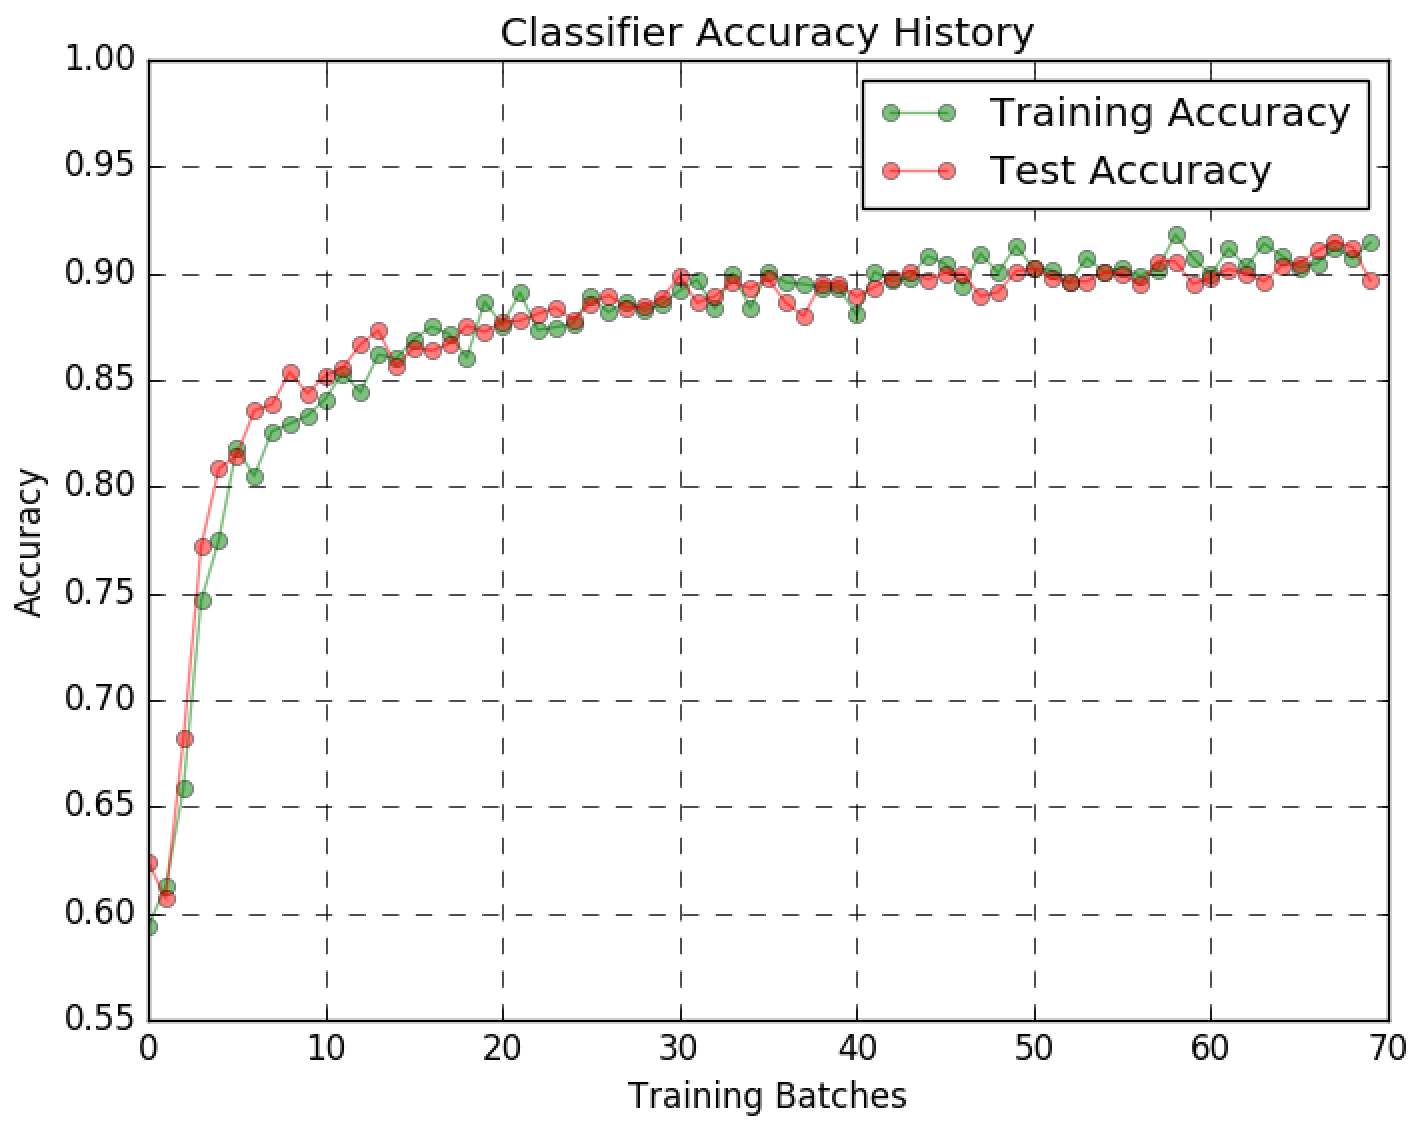
\includegraphics[width=0.45\textwidth]{Images/Calo/accuracy_large_window.png}
    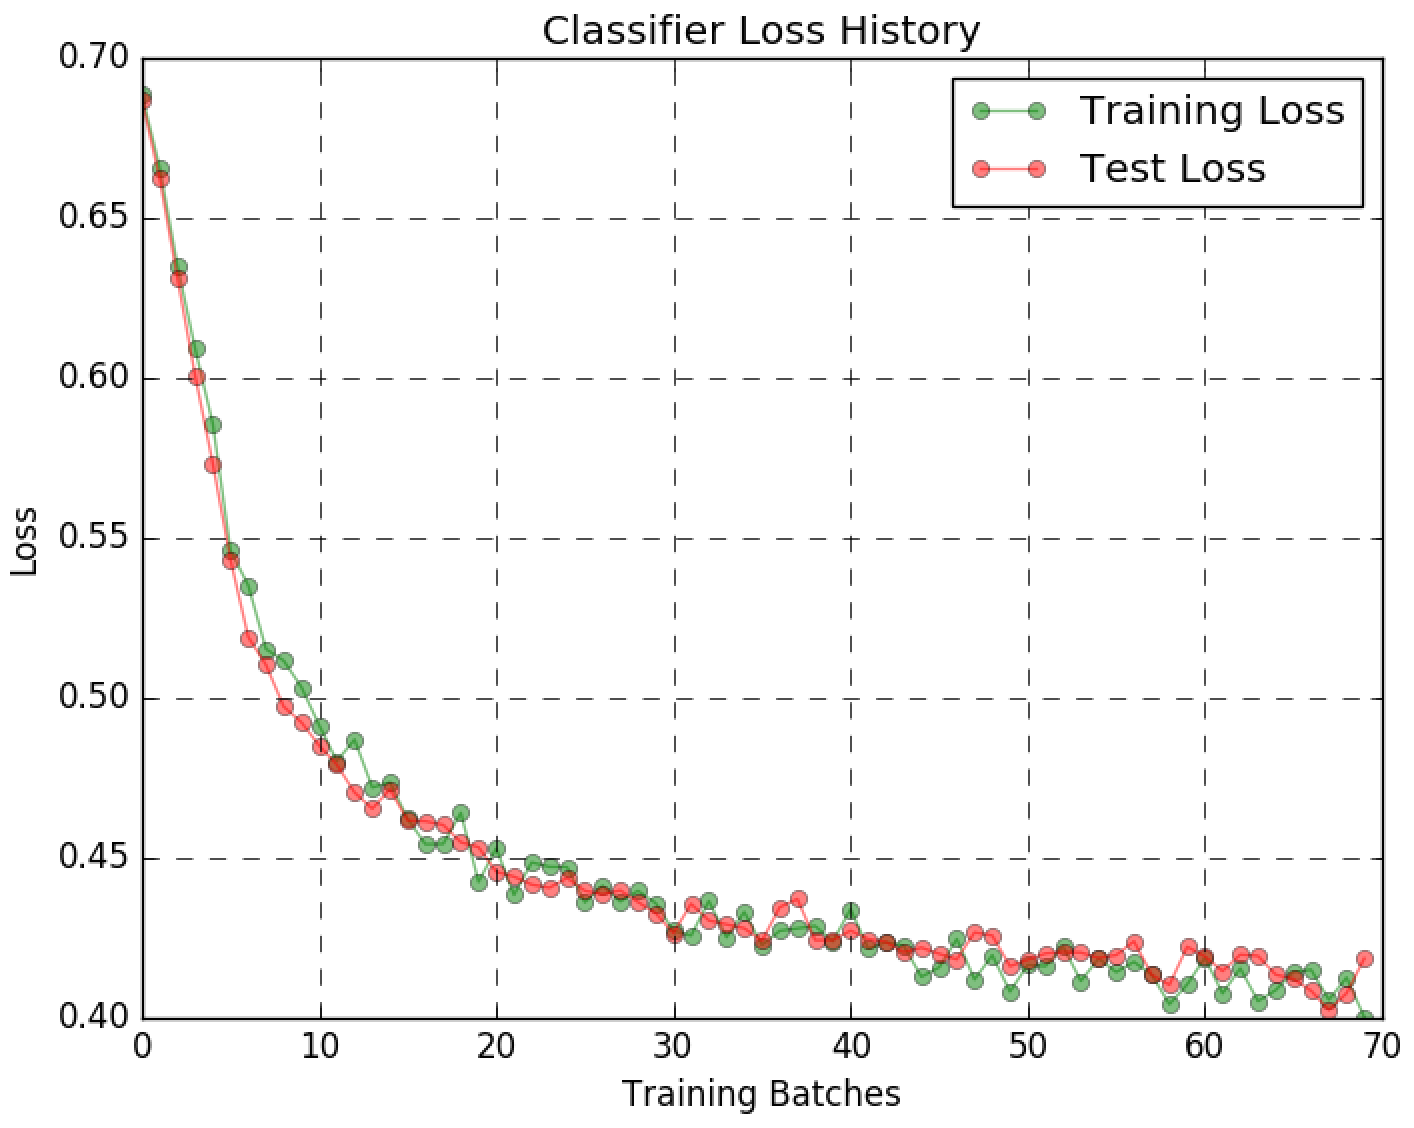
\includegraphics[width=0.45\textwidth]{Images/Calo/loss_large_window.png}
    \caption{Training history for different choices of the input 3D array zise: Accuracy (left) and loss (right) as a function of the training batch for photon/neutral pion classification, using a 25x25x25 (top) and 51x51x25 (bottom) ECAL window size.\label{fig:classification_window}}
\end{figure*}